\begin{frame}
\frametitle{Success Stories}
\begin{itemize}
\item Some examples which show impact of CP
\item Not just a nice model or a novel constraint
\item Impact of solution
\item Recognition of CP as best tool for the job
\end{itemize}
\end{frame}

\section{Rosetta/Philae Mission Scheduling, LAAS-CNRS}

\begin{frame}
\frametitle{Scheduling of Data Transfer on Philae Lander}
\begin{columns}
\begin{column}{0.5\textwidth}
\begin{itemize}
\item Rosetta/Philae Mission 2004-2014
\item Land on a comet
\item Perform experiments
\item How do the data get back to earth?
\end{itemize}
\end{column}
\begin{column}{0.5\textwidth}
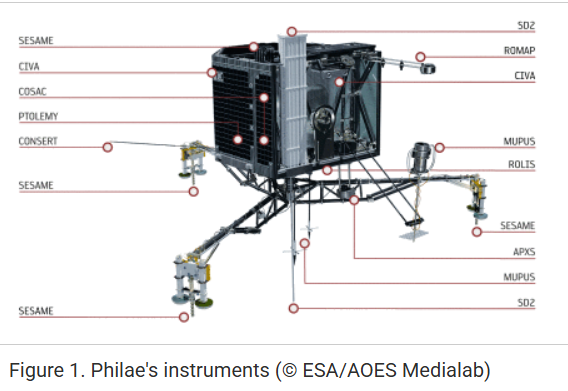
\includegraphics[width=\textwidth]{../summerschool2026/images/philae}
\end{column}
\end{columns}
\end{frame}

\begin{frame}
\frametitle{CP on a Comet?}
\begin{itemize}
\item Constraint model schedules data transfers between Rosetta (orbiter) and Philae (lander)
\item Part of the software suite controlling the lander
\item Developed by LAAS-CNRS, Toulouse
\begin{itemize}
\item Running on earth, not in the lander!
\end{itemize}
\item Written in Ilog Scheduler
\item To learn more: Simonin et al, 2015: Scheduling scientific experiments for comet exploration
\item Also: ACP Website \url{https://www.a4cp.org/node/1058}
\end{itemize}
\end{frame}

\begin{frame}
\frametitle{Global Constraint Model}
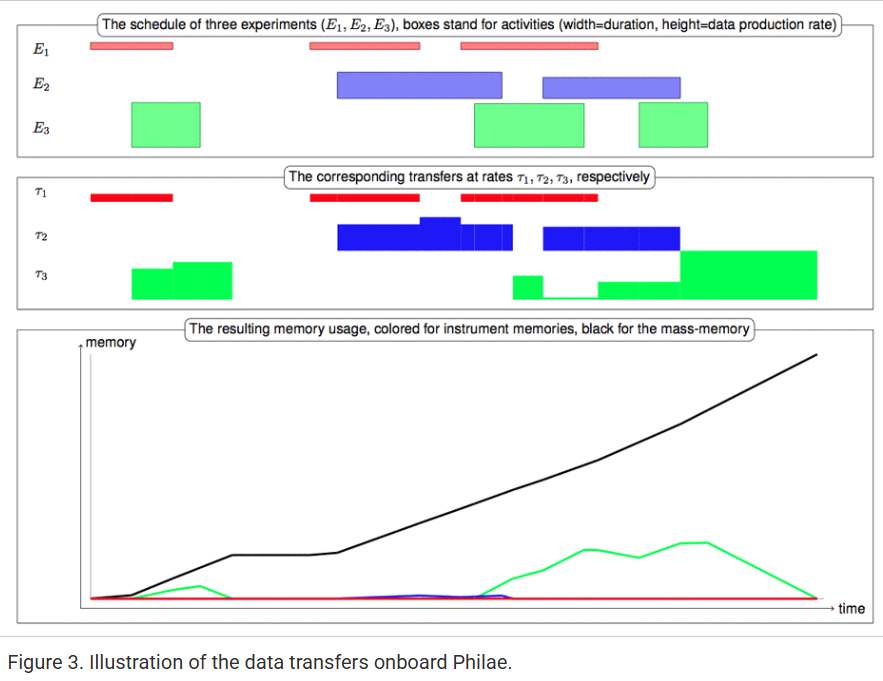
\includegraphics[width=9cm]{../summerschool2026/images/philaedatatransfer}
\end{frame}

\begin{frame}
\frametitle{Rosetta/Philae in popular culture}
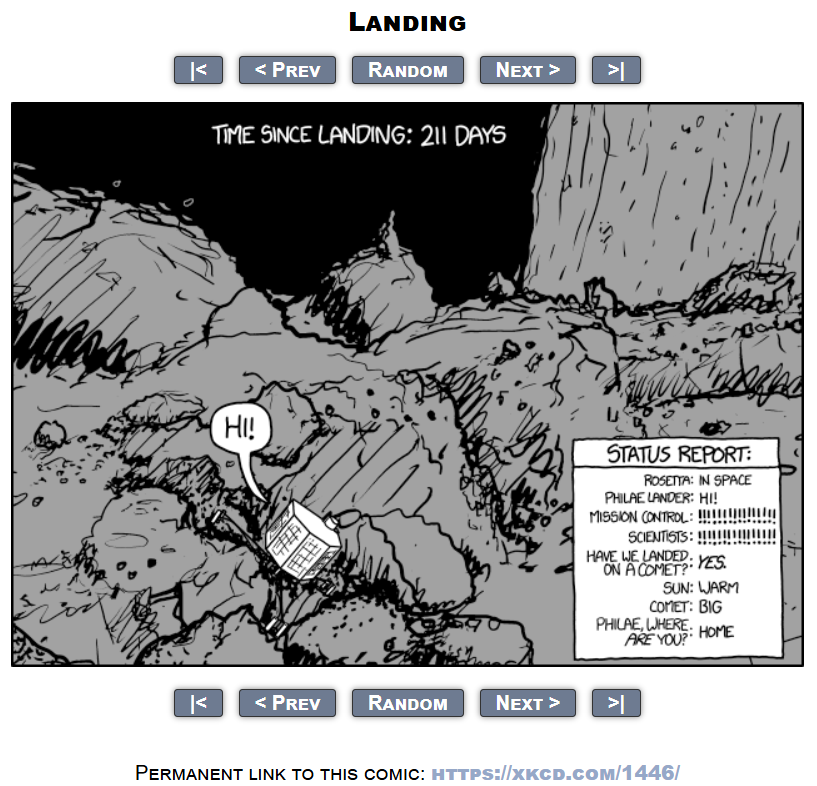
\includegraphics[width=7cm]{images/xkcd1446}
\end{frame}

\section{Unison Compiler, SICS, KTH, Ericsson, 2010-2018}

\begin{frame}
\frametitle{Unison}
\begin{itemize}
\item Long-term project to develop CP Based optimising compiler
\begin{itemize}
\item Instruction selection
\item Register allocation
\item Instruction scheduling
\end{itemize}
\item Integrates in \href{http://llvm.org}{LLVM} toolchain
\item Targeted for embedded systems processors
\end{itemize}
\end{frame}

\begin{frame}
\frametitle{What is the problem?}
\begin{itemize}
\item Translate high-level language into assembly code
\item Map variables to registers and memory
\item Map statements to instruction sequences
\item Modern processors are powerful, but complicated!
\item Complex resource allocation and scheduling problem
\item Most compact/ most performant code?
\item Must work all the time
\item Improvements are shared by all users (huge impact)
\end{itemize}
\end{frame}

\begin{frame}
\frametitle{Example High-level Program}
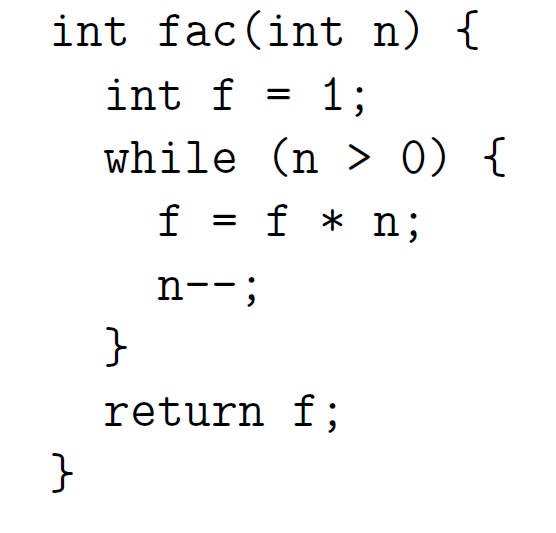
\includegraphics[width=6cm]{../summerschool2026/images/unisonexample}

\end{frame}

\begin{frame}
\frametitle{Generated Code Comparison (subtle)}
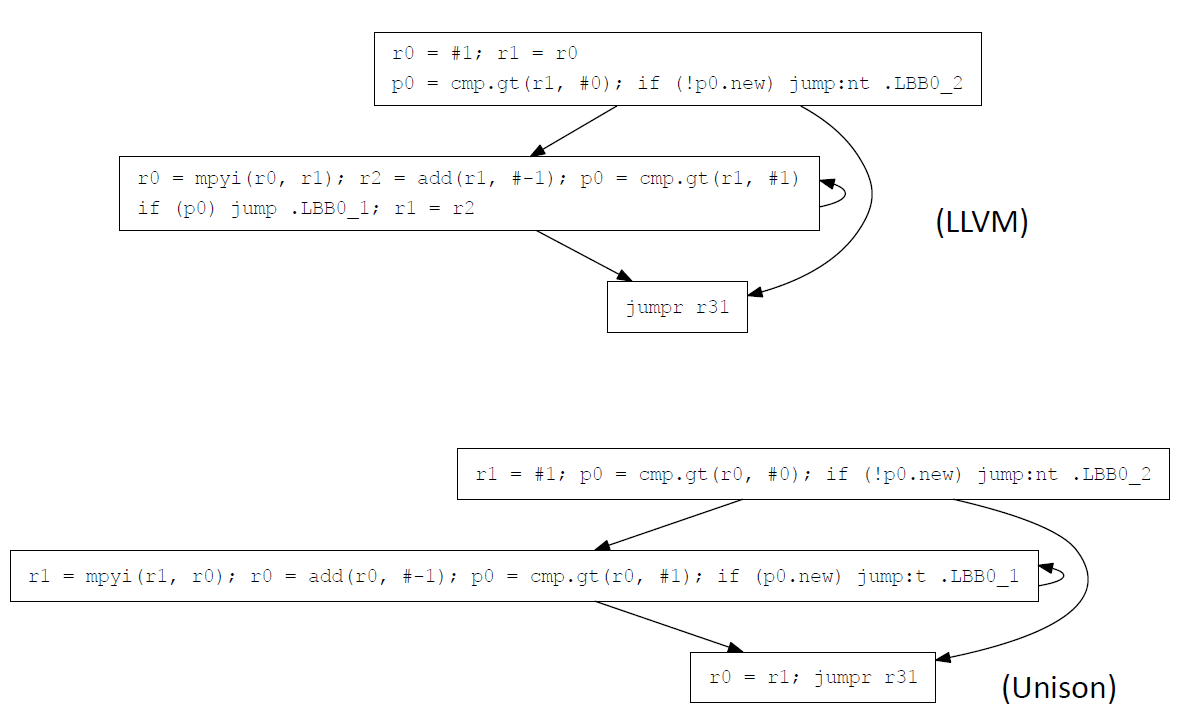
\includegraphics[width=10cm]{../summerschool2026/images/unisoncode}
\end{frame}

\begin{frame}
\frametitle{Unison Speedup Compared to LLVM}
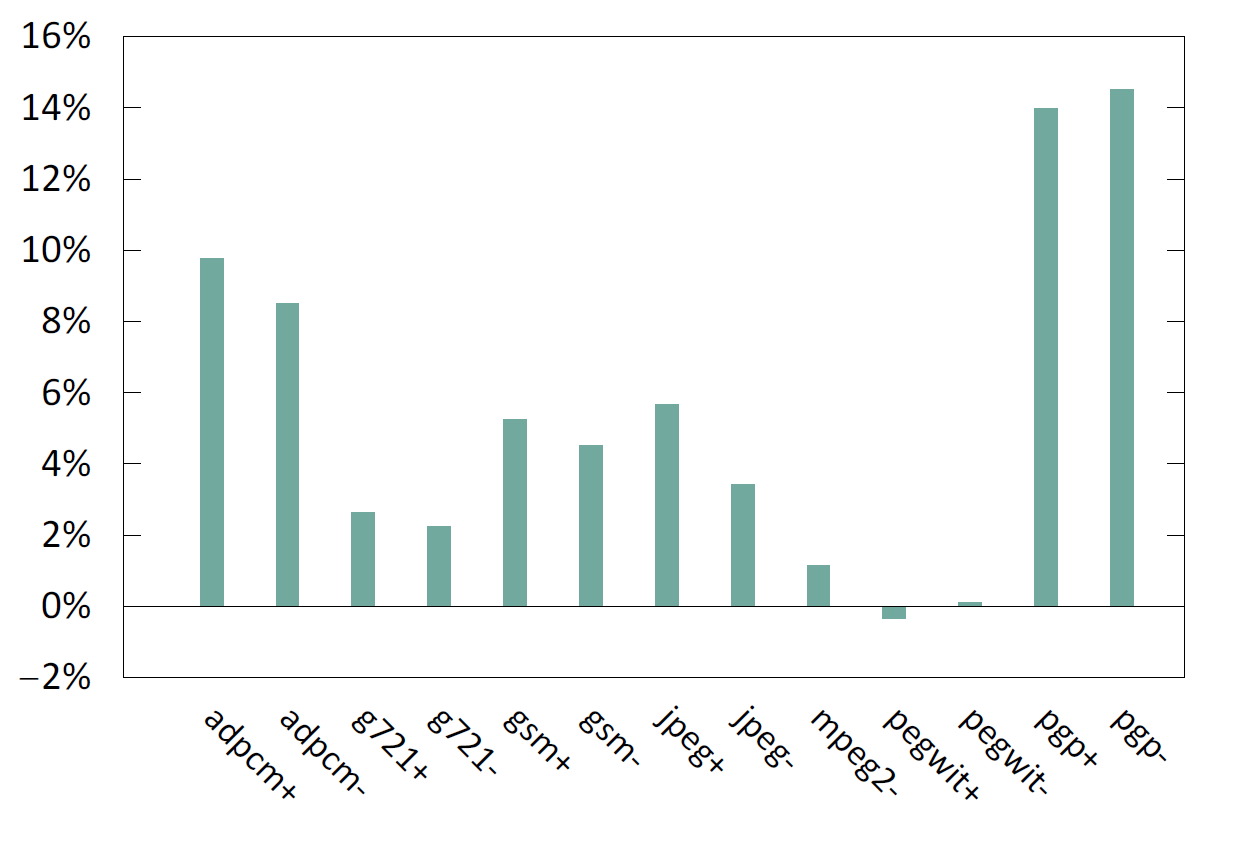
\includegraphics[width=10cm]{../summerschool2026/images/unisonspeedup}
\end{frame}

\begin{frame}
\frametitle{Conclusions}
\begin{itemize}
\item State-of-the-art compiler
\item Multiplier effect of improvements, everybody wins!
\item Significant number of publications outside CP domain
\item To learn more: Roberto Castaneda Lozano, NordConsNet 2025: Working in Unison with Mats \url{https://pierre-flener.github.io/research/NordConsNet/NordConsNet25/}
\end{itemize}
\end{frame}


%\section{Molecular Design, Thomas Schiex CP 2023}

%\section{Workforce Rostering, IBM Haifa, CP 2011}
